\titleformat{\chapter}[display]{\bfseries\centering}{\huge Chapter \thechapter}{1em}{\Huge #1}
\newgeometry{top=3cm, bottom=2.2cm, left=3cm, right=2cm, headsep=1.2cm, footskip=1cm, headheight=0.3cm, textheight=24.5cm, textwidth=16cm}
\onehalfspacing

\pagestyle{fancy}
\fancyhf{}
\renewcommand{\headrulewidth}{0pt}
\lhead{Chapter 1}
\rhead{Introduction}
\cfoot{\thepage}
\chapter{Introduction}

\section{Introduction}
\noindent Social media platforms carry job offers, scholarship notices, messages from classmates and links to external services. The same channels are used for fraud and abuse: a fake placement offer may demand a ``registration fee'' or a one-time password (OTP), a link may imitate a trusted login page, an account may be fake or automated, and a conversation may contain directed insults or threats. Protection depends largely on manual reporting and platform rules, and the volume of activity makes manual detection slow and inconsistent.\\

\noindent Sentinel addresses this problem from the side of the individual user. The user decides what to check and supplies only what is in front of them: a message, a link, the preceding turns of a conversation, or visible profile facts. Sentinel returns three separate assessments (fraud, harmful content and profile), states which checks were unavailable, and suggests a next step. It never describes an unlisted link as ``safe'' or an unusual account as ``fake''. The project has two strands: a usable local application and a reproducible machine-learning (ML) research pipeline, in which a learned model is released into the application only when a held-out evaluation, judged against a gate fixed in advance, supports it. The application now covers four threats: scam and phishing messages (rules plus a learned scam-text model), harmful and dangerous language (an English and Hinglish rule engine), automated or fake accounts (an explainable bot-detection module that uses only official APIs or user-supplied data) and new scam campaigns (a privacy-preserving community network). Besides on-demand checks, the Chrome extension can scan the visible text of sites the user opts in to. This report covers the work completed in Semester VII.

\section{Background Study: Terminologies and Definitions}
\begin{itemize}
\item \textbf{Phishing / smishing:} social-engineering messages that persuade a victim to reveal credentials, OTPs or payment details, usually through a link to an imitation website (smishing: by SMS or chat).
\item \textbf{Fake account / social bot:} an account that misrepresents who operates it, or that is operated automatically \cite{lit3}.
\item \textbf{Directed abuse / cyberbullying:} insults, threats or harassment aimed at a person; establishing bullying usually needs context such as the target and repetition \cite{cad}.
\item \textbf{Punycode and homograph attacks:} internationalised domain names are encoded as \texttt{xn--} labels; look-alike characters can make a malicious domain appear identical to a trusted one \cite{homograph}.
\item \textbf{Public Suffix List (PSL):} a list of suffixes such as \texttt{.co.in} used to find a URL's registrable domain \cite{psl}; Sentinel uses it to keep related URLs in the same data split.
\item \textbf{Reputation feed:} a list of verified phishing URLs such as PhishTank \cite{phishtank}; an absent URL is \emph{unlisted}, not proven safe.
\item \textbf{TF-IDF, logistic regression, gradient boosting, Naive Bayes:} standard text features and classifiers \cite{sklearn}; \textbf{DistilBERT} is a compact transformer language model \cite{distilbert}.
\item \textbf{Calibration:} mapping raw model scores to probabilities that match observed frequencies \cite{platt,guo}.
\item \textbf{Data leakage / grouped splitting:} leakage occurs when related items (same domain, thread or author) appear in both training and test data; grouped splitting keeps each group in one partition.
\item \textbf{Temperature scaling and isotonic regression:} calibration methods that divide a network's logits by a fitted temperature $T$ \cite{guo}, or map scores through a fitted monotone step function \cite{zadrozny}.
\item \textbf{MinHash and locality-sensitive hashing (LSH):} MinHash estimates the Jaccard similarity of two sets from short signatures \cite{broder}; LSH groups signatures into bands so that similar items collide with high probability \cite{mmds}. Sentinel uses them to recognise reworded scams without storing their text.
\item \textbf{$k$-anonymity:} a release rule under which a record is published only when it cannot be tied to fewer than $k$ individuals \cite{sweeney}; Sentinel publishes a scam campaign only after $k=5$ distinct reporters.
\item \textbf{Social bot detection and cross-dataset evaluation:} classifiers that separate automated from human accounts; scores on mixed data overstate accuracy, so models are tested on whole datasets or bot families held out from training \cite{yang2020,cresci2017}.
\item \textbf{ONNX:} a portable format for trained neural networks that ONNX Runtime executes on a CPU without the training framework \cite{onnx}.
\item \textbf{Manifest V3 and HMAC:} the current Chrome extension platform \cite{mv3}, and a keyed hash used to authenticate data \cite{hmac}.
\end{itemize}

\section{Fundamental Study Points of the Selected Topic and Domain}
\begin{enumerate}
\item \textbf{Threats arrive together:} one suspicious post can combine a persuasive message, a link and an account, each carrying different evidence.
\item \textbf{Users see only part of the picture:} an ordinary user cannot see login logs, IP addresses or full posting histories, so methods that need platform data \cite{lit2} cannot be used directly.
\item \textbf{Rules are explainable but narrow:} indicators such as ``asks for an OTP'' are easy to explain but miss new wording and formats.
\item \textbf{Learned models need careful evaluation:} leakage or class-collection bias can produce high scores that do not transfer.
\item \textbf{False alarms carry a cost:} phishing is rare, so even a small false-positive rate produces many false warnings.
\end{enumerate}

\section{Identification of Challenges in the Selected Topic}
\begin{itemize}
\item \textbf{Data and label meaning:} genuine, permissioned social-media message--link pairs are scarce, and spam labels must not be relabelled as phishing.
\item \textbf{Source and format bias:} if the classes were collected differently, a model learns the format instead of the threat (Section~\ref{sec:v1res}).
\item \textbf{Privacy and safe link handling:} messages may contain personal data, and visiting a suspicious link is unsafe, so analysis must be local and work from the URL string alone.
\item \textbf{Code-mixed and disguised language:} Indian users write in English, Hinglish and transliterated Hindi, and abusers disguise words (\texttt{1d10t}, \texttt{k.y.s}, stretched letters), which defeats naive keyword lists.
\item \textbf{Platform rules for account data:} scraping profiles breaks platform terms, so bot detection must use official APIs or data the user supplies, and must handle missing data honestly.
\item \textbf{Limited hardware:} student laptops (Ryzen 7 7435HS, 16 GiB RAM, RTX 3050 with 4 GiB VRAM; Apple M4) constrain model size and training memory, so the served models must run on a CPU.
\end{itemize}

\section{Motivation}
\noindent Students are frequent targets of fake internship offers that ask for fees or codes, and of links that imitate college or banking portals. Existing research usually handles one threat at a time and often relies on platform data, while consumer tools give a verdict without explaining it. The team wanted a tool a student could use before replying to a suspicious post: local, covering the common threats, explaining what it observed and what it could not check, and honest about the limits of its models.

\section{Problem Statement and Proposed Solution}
\noindent\textbf{Problem statement.} Social media users are increasingly exposed to fake accounts, phishing links, and cyberbullying or toxic content, which can lead to fraud, privacy risks, harassment and loss of trust. Existing mechanisms rely heavily on manual moderation or separate security tools, making timely detection difficult for an ordinary user. An explainable system is needed that analyses supplied profiles, URLs and content and identifies potential threats using rules, Machine Learning and Natural Language Processing (NLP), without exposing the user's data or overstating its certainty.\\

\noindent\textbf{Objectives.}
\begin{enumerate}
\item Let a user check a post, link, conversation, profile details or social-media account on demand from a web app or Chrome extension, without a cloud account.
\item Report fraud, harmful-content, learned-model, community and account observations separately, with evidence, unavailable checks, uncertainty and a suggested action.
\item Detect harmful and dangerous language (threats, self-harm risk, sextortion, harassment) in English and Hinglish, and give supportive advice for self-harm.
\item Warn users while they browse, only on sites they opt in to, by marking risky visible text on the page.
\item Estimate whether an account behaves like a bot using only official APIs or user-supplied data, and show which signals drove the estimate.
\item Let users protect each other from new scam campaigns without sharing message text.
\item Store a case only on explicit request, with feedback, JSON export and deletion.
\item Build a reproducible ML pipeline and evaluate models only on held-out data with unseen domains, threads, datasets or bot families, release a model only after it passes a gate fixed in advance, and answer: \emph{does combining message and URL evidence improve phishing-request detection on unseen domains at an acceptable false-positive rate?}
\end{enumerate}

\noindent\textbf{Proposed solution.} Sentinel consists of a local \textbf{application} and a \textbf{research pipeline}. The application is a standard-library Python HTTP API bound to 127.0.0.1, a four-page web client (check content, bot accounts, community network and saved cases) and a Manifest V3 Chrome extension with on-demand checks and opt-in auto-scan. It runs evidence rules for messages and URLs with an optional verified phishing feed, a harmful-language rule engine, a calibrated scam-text model (text-ml-v2), a community-campaign matcher, profile indicators and a bot-detection module. The research pipeline trains and evaluates models under a leakage-aware protocol. Each learned model reports in its own field and is shown live only after passing its release gate; models that failed (the URL models and the profile-only bot model) stay in research. Figure~\ref{fig:block} gives the general block diagram.

\begin{figure}[H]
\centering
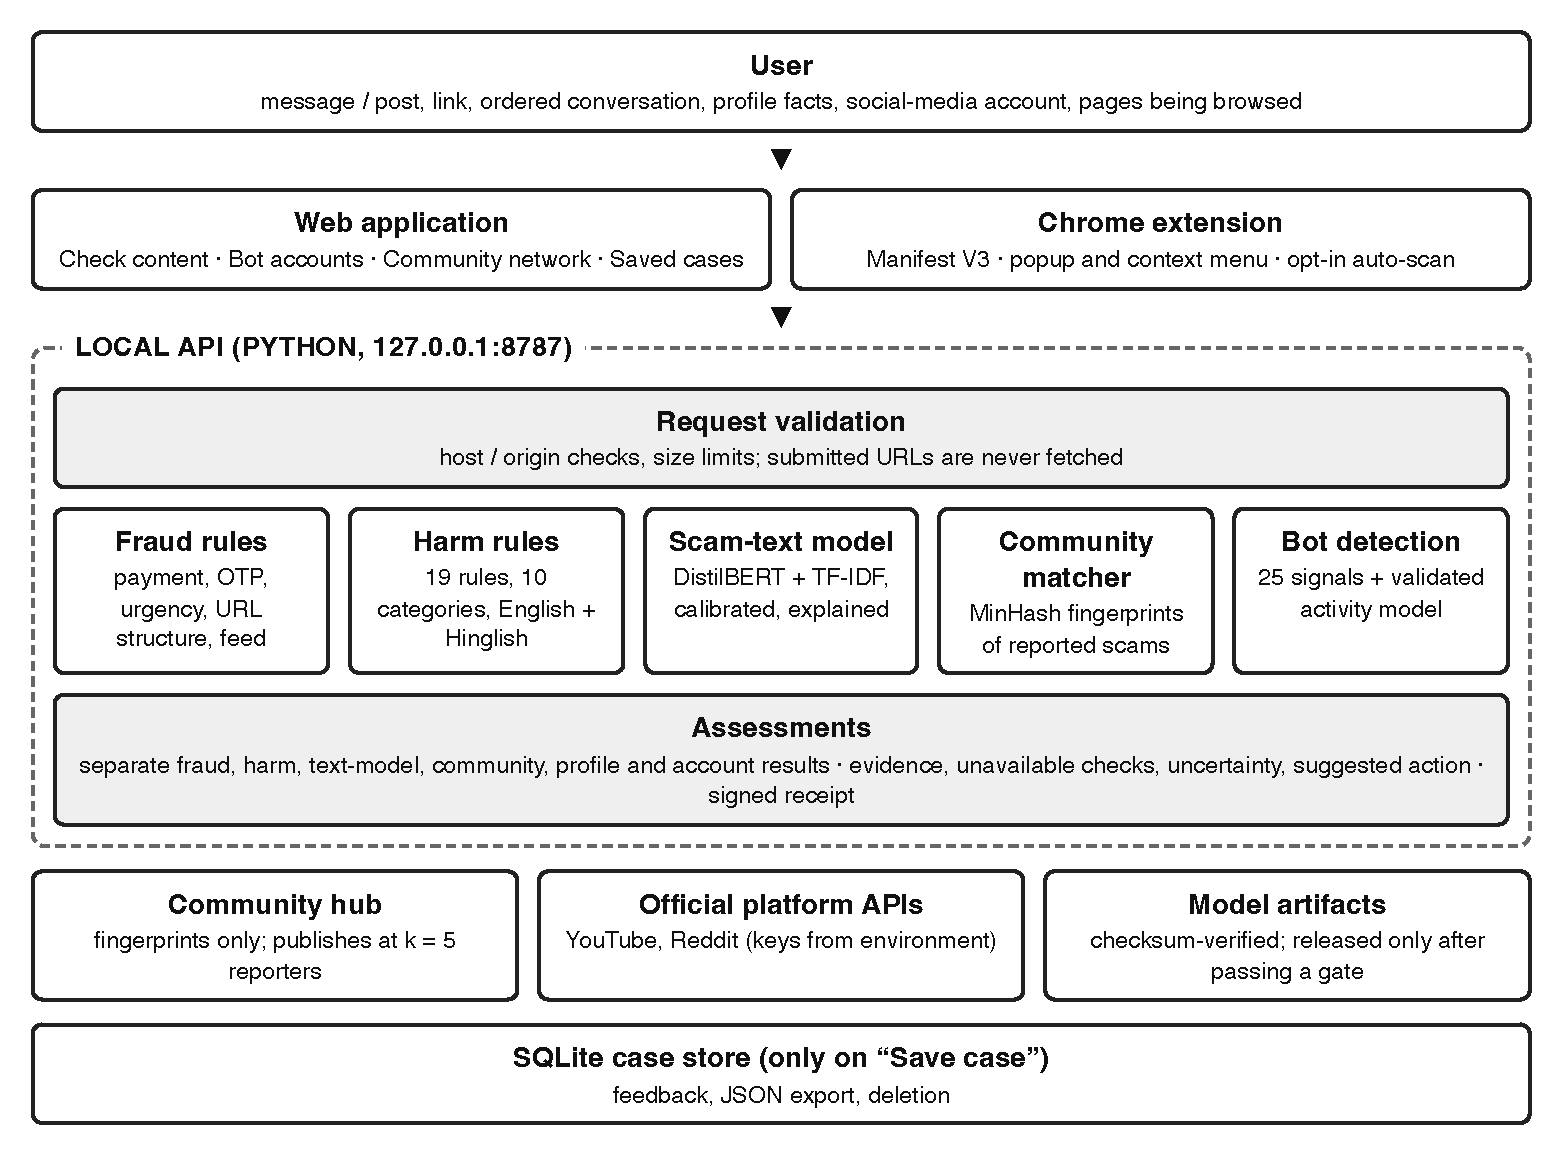
\includegraphics[width=0.86\linewidth]{dia2/block_v2.pdf}
\caption{General block diagram of Sentinel}
\label{fig:block}
\end{figure}

\noindent\textbf{Organization of the report.} Chapter 2 surveys existing work, Chapter 3 presents the proposed system and its design, Chapter 4 the implementation plan and experimental setup, Chapter 5 the results, Chapter 6 the conclusion and Chapter 7 the references.
